\section{仿真平台测试 }
在Gazebo中载入两个仿生机器鼠模型,分别用不同颜色标识,表示在实验环境中交互的个体(图\ref{figure_setup})。针对在Gazebo中开展多体仿真的需求,ROS提供了命名空间(ns)用以区分不同的机器人。具体而言,处于同一命名空间的机器鼠将共享话题、服务和动作,而不同命名空间的机器鼠之间解耦。
\begin{figure}[htb]
  %\vspace{13pt}
  \centering
  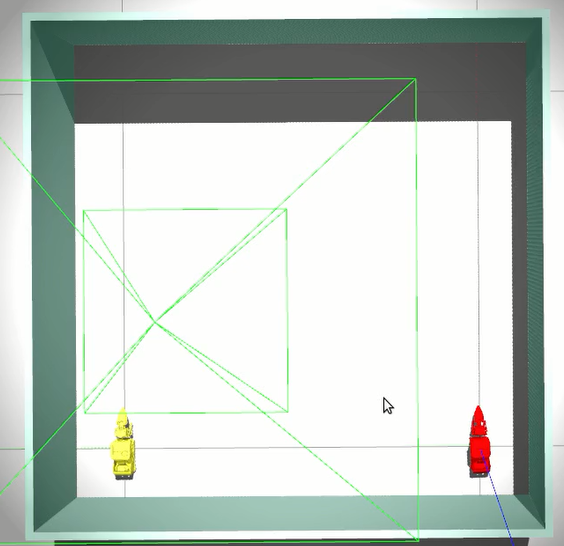
\includegraphics[width=0.5\linewidth]{images/ch03/setup.png}
  \caption{Gazebo仿真界面启动}\label{figure_setup}
\end{figure}

为测试仿真平台工作的可靠性,本文编写了读取键盘输入的脚本程序,利用键盘作为操作器,调用动作执行层的接口函数,对同时载入两个仿生机器鼠模型仿真平台进行了操作测试,测试内容包括对机器鼠模型在仿真环境中的轮部运动和躯干运动。

\subsection{轮部运动测试}
在直线运动方面,机器鼠能够表现与生物鼠相似的特性。控制仿生机器鼠接近其交互伙伴,使其做出与图\ref{figure_appr}相似的动作,其表现如图\ref{figure_simappr}。
\begin{figure}[htbp]
  %\vspace{13pt}
  \centering
  \subfigure[$t_0$]{\label{figure_simappr_0000}
  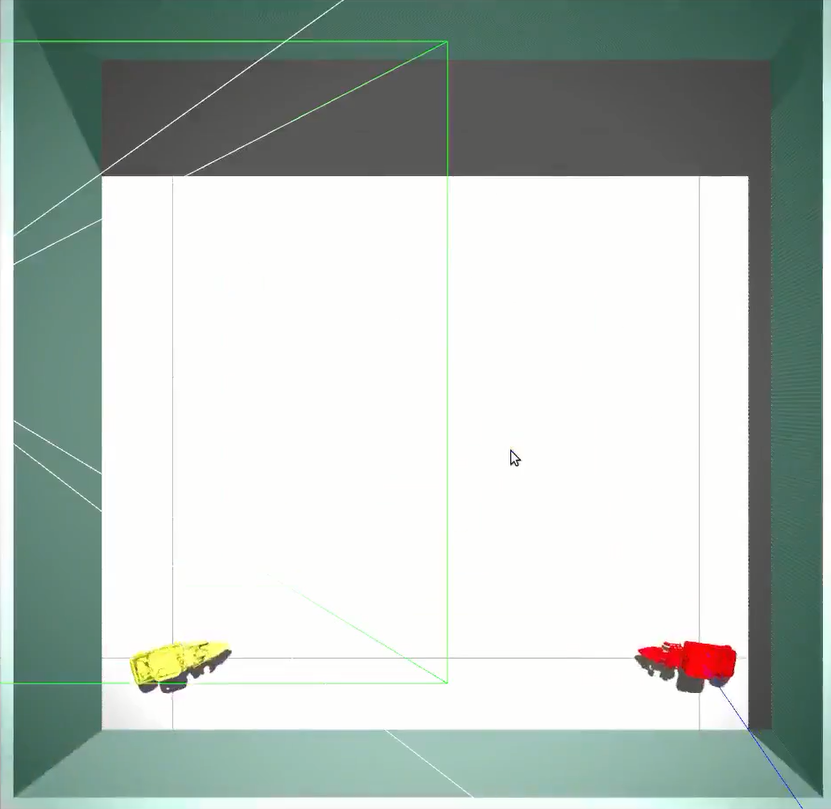
\includegraphics[width=0.27\linewidth]{images/ch03/check/walk/t000.png}
  }
  \subfigure[$t_0+685~ms$]{\label{figure_simappr_0525}
  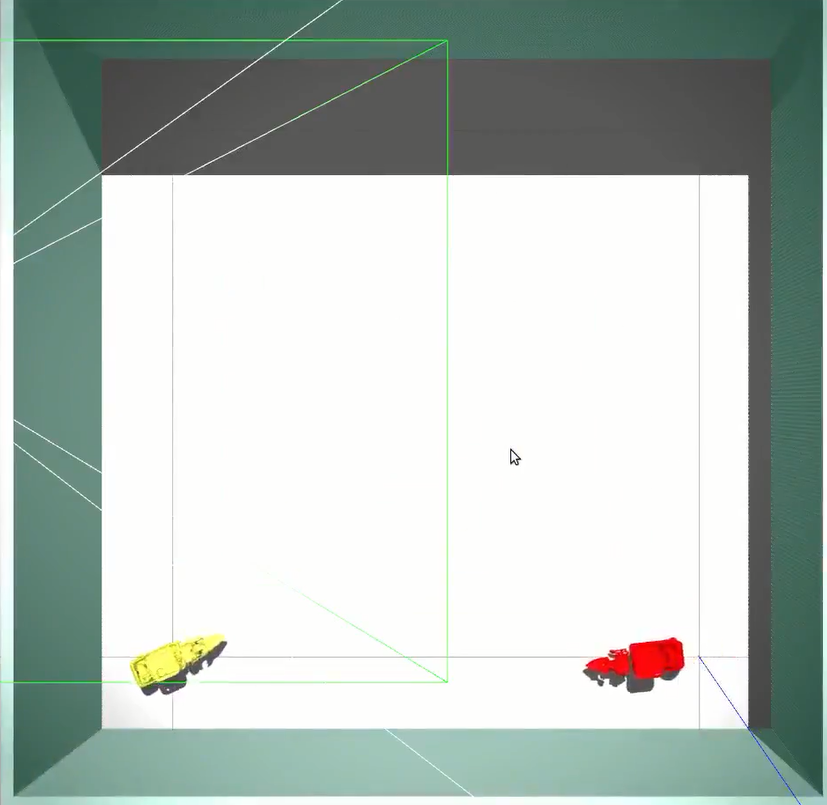
\includegraphics[width=0.27\linewidth]{images/ch03/check/walk/t001.png}
  }
  \subfigure[$t_0+1324~ms$]{\label{figure_simappr_1724}
  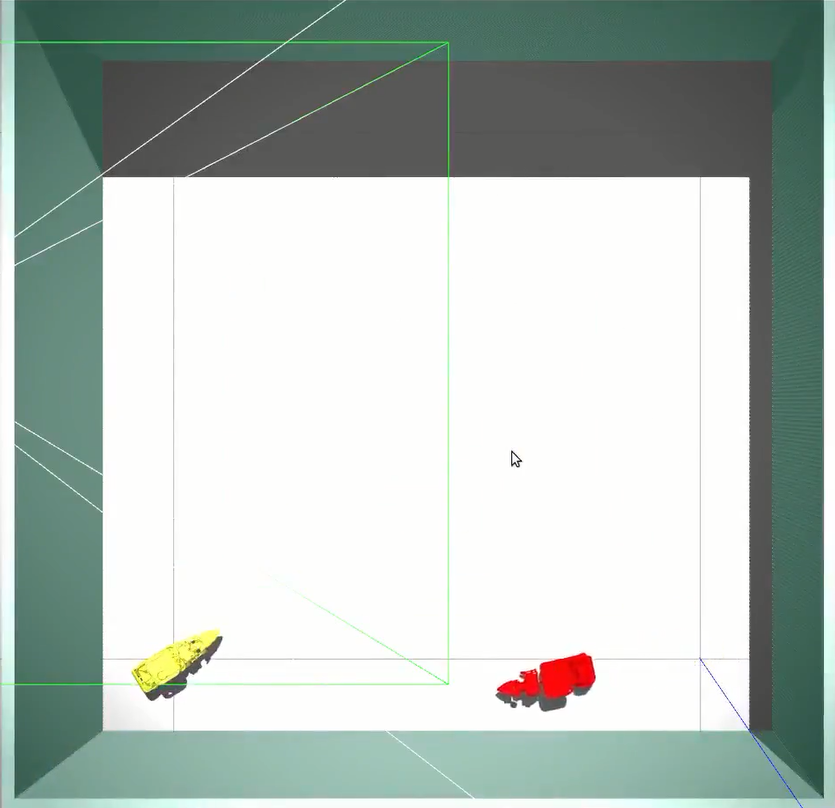
\includegraphics[width=0.27\linewidth]{images/ch03/check/walk/t002.png}
  }\\
  \subfigure[$t_0+1975~ms$]{\label{figure_simappr_2225}
  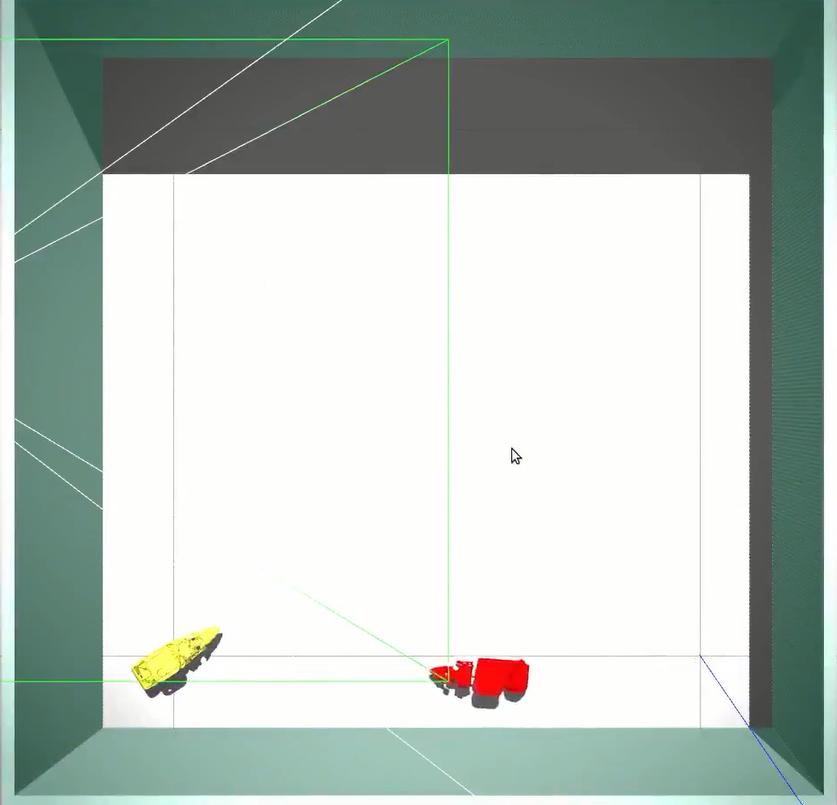
\includegraphics[width=0.27\linewidth]{images/ch03/check/walk/t003.png}
  }
  \subfigure[$t_0+2621~ms$]{\label{figure_simappr_2721}
  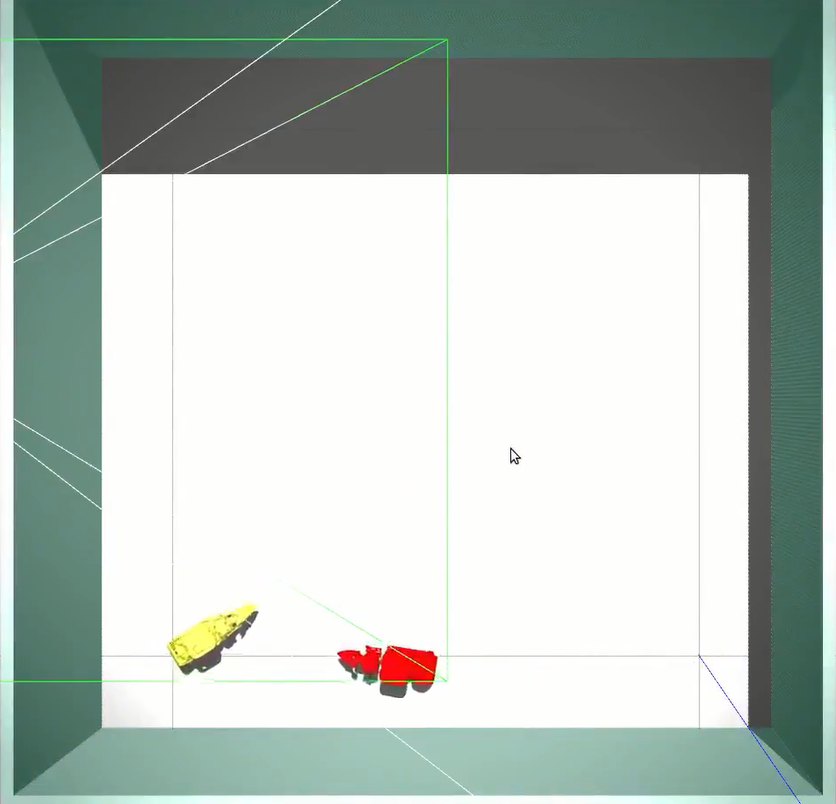
\includegraphics[width=0.27\linewidth]{images/ch03/check/walk/t004.png}
  }
  \subfigure[$t_0+3214~ms$]{\label{figure_simappr_3214}
  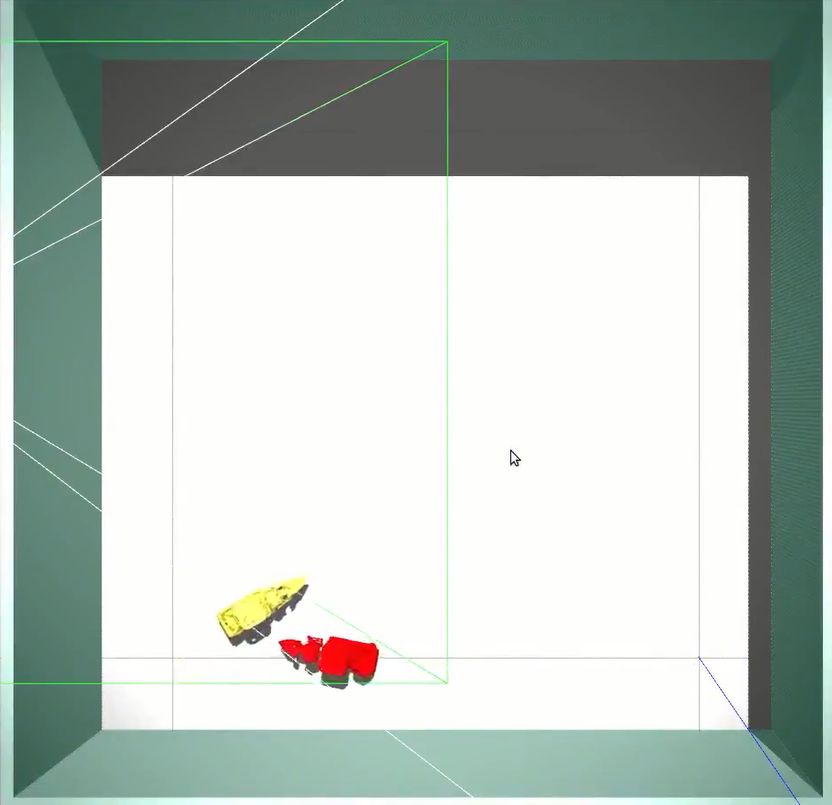
\includegraphics[width=0.27\linewidth]{images/ch03/check/walk/t005.png}
  }
  \caption{Gazebo中机器鼠(红)接近其交互伙伴}\label{figure_simappr}
\end{figure}
相比之下,虽然机器鼠的启动速度略慢于生物鼠,但在总体上机器鼠直线接近交互伙伴的速度与生物鼠相近。同时,在引入机器鼠角速度作为反馈后,机器鼠模型能够克服不同部位摩擦力不同产生的影响,运动轨迹保持为直线。

在转向方面,机器鼠同样能在相近的时间内完成方向调整,过程如图\ref{figure_simturn}。
\begin{figure}[htb]
  %\vspace{13pt}
  \centering
  \subfigure[$t_0$]{\label{figure_simturn_00-1}
  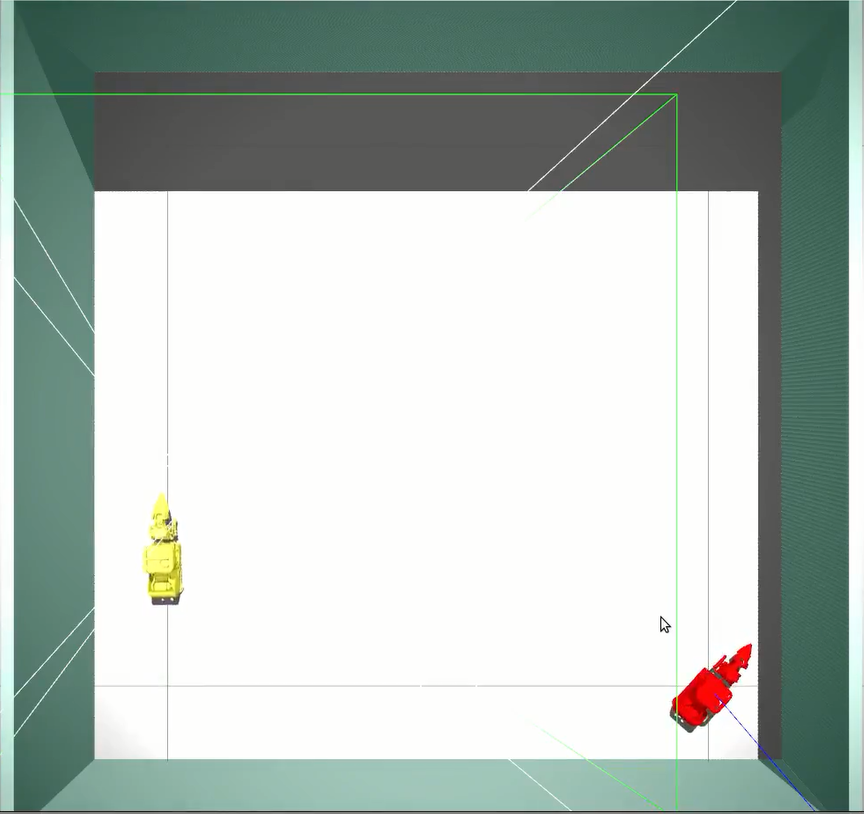
\includegraphics[height=0.27\linewidth]{images/ch03/check/turn/-1.png}
  }
  \subfigure[$t_0+427~ms$]{\label{figure_simturn_0000}
  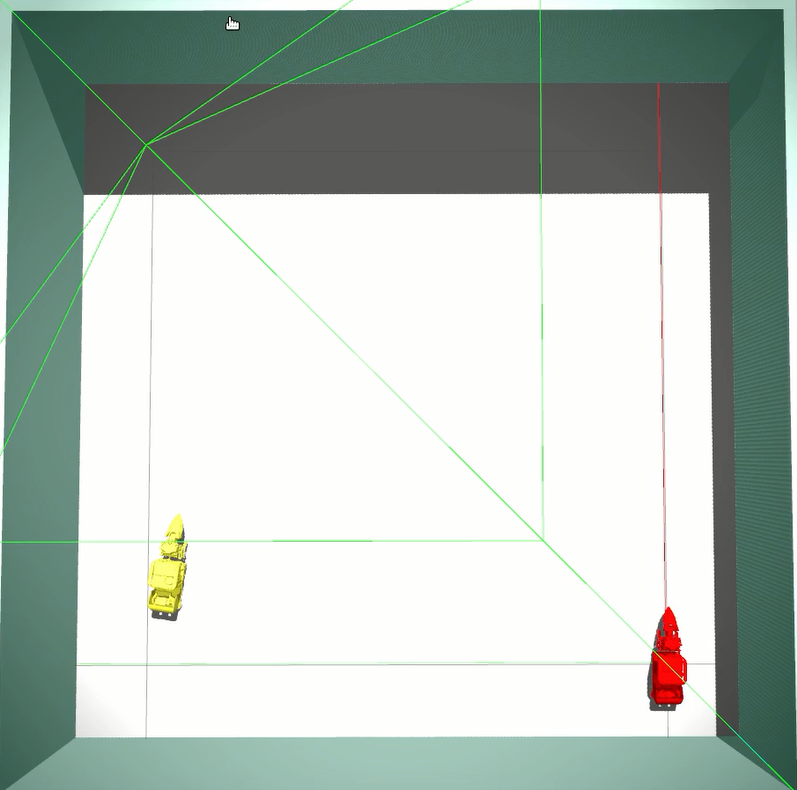
\includegraphics[height=0.27\linewidth]{images/ch03/check/turn/0.png}
  }
  \subfigure[$t_0+850~ms$]{\label{figure_simturn_0430}
  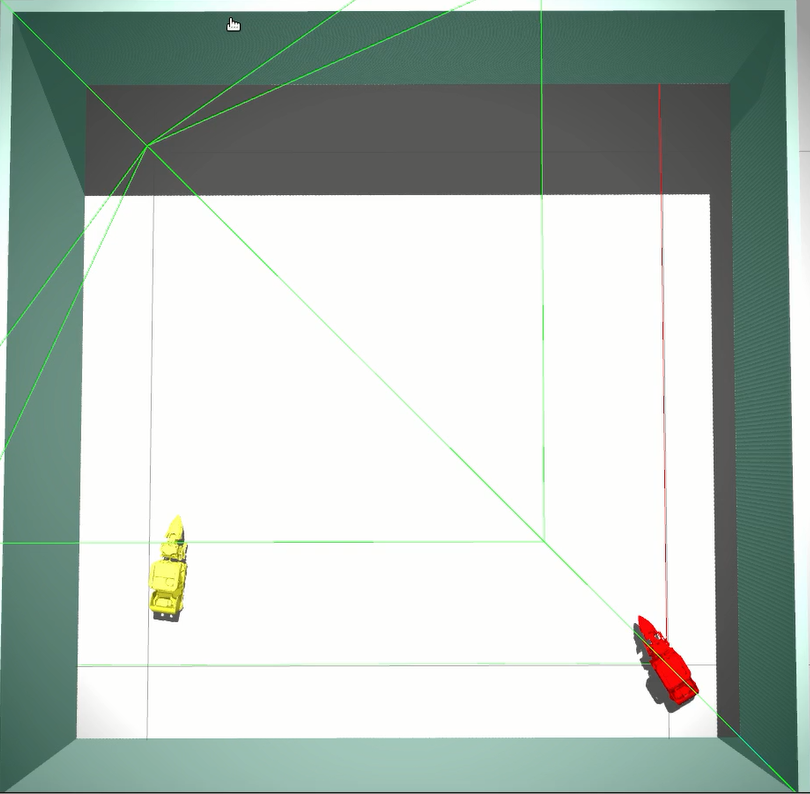
\includegraphics[height=0.27\linewidth]{images/ch03/check/turn/1.png}
  }\\
  \subfigure[$t_0+1252~ms$]{\label{figure_simturn_0950}
  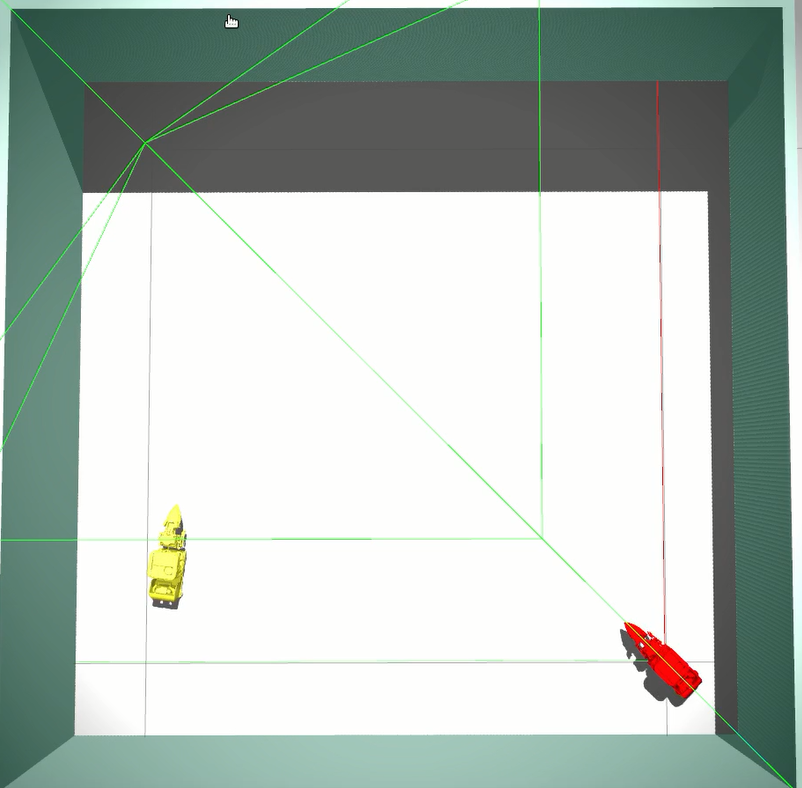
\includegraphics[height=0.27\linewidth]{images/ch03/check/turn/2.png}
  }
  \subfigure[$t_0+1721~ms$]{\label{figure_simturn_1721}
  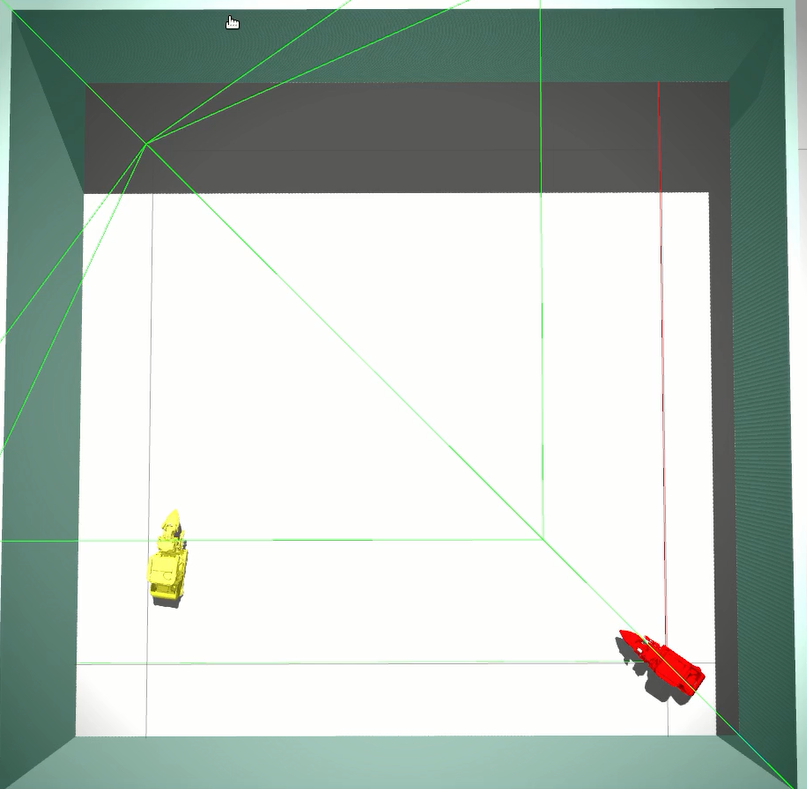
\includegraphics[height=0.27\linewidth]{images/ch03/check/turn/3.png}
  }
  \subfigure[$t_0+2250~ms$]{\label{figure_simturn_2250}
  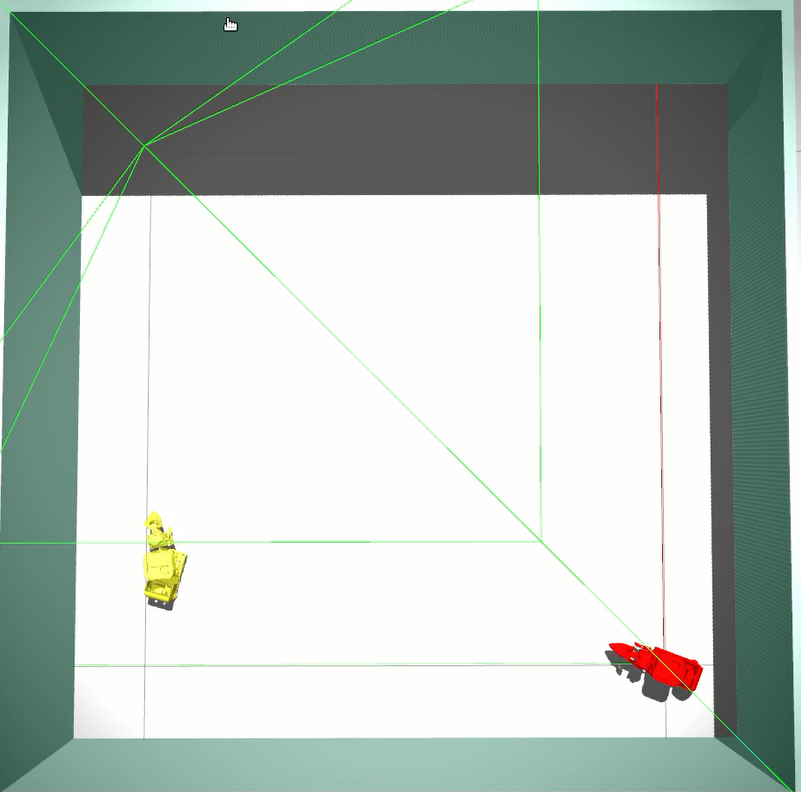
\includegraphics[height=0.27\linewidth]{images/ch03/check/turn/4.png}
  }
  \caption{Gazebo中生物鼠(红)左转}\label{figure_simturn}
\end{figure}

上述分析表明仿真平台对仿生机器鼠模型轮部运动的控制能够实现仿鼠移动,这为其产生接近、远离等需要位置变化的行为提供了条件。
\subsection{躯干运动测试}
对仿鼠机器鼠躯干部分运动所涉及的七自由度机械臂的评估从运动速度和运动精度两方面判定。在运动速度方面,将仿生机器鼠在仿真平台中执行相应动作耗费时间与生物鼠对比;在运动精度方面,通过设定仿生机器鼠运动的允许误差,观测平台运行稳定性。

运动速度的测试主要考虑机器鼠完成一次姿态切换花费的时间,以其从初始姿态运动至直立姿态为例,其过程如图\ref{figure_simtorear}所示。
\begin{figure}[htb]
  %\vspace{13pt}
  \centering
  \subfigure[$t_0$]{\label{figure_simtorear_0000}
  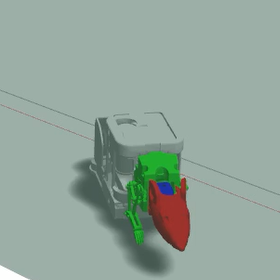
\includegraphics[width=3.0cm]{images/ch03/check/torear/0000.png}
  }
  \subfigure[$t_0+333~ms$]{\label{figure_simtorear_0333}
  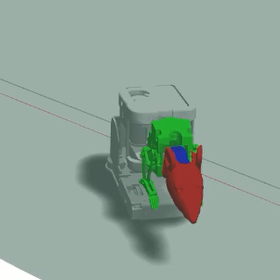
\includegraphics[width=3.0cm]{images/ch03/check/torear/0333.png}
  }
  \subfigure[$t_0+658~ms$]{\label{figure_simtorear_0658}
  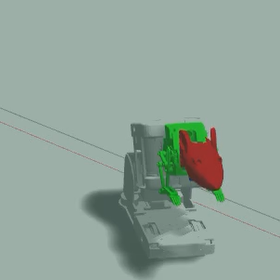
\includegraphics[width=3.0cm]{images/ch03/check/torear/0658.png}
  }
  \subfigure[$t_0+984~ms$]{\label{figure_simtorear_0984}
  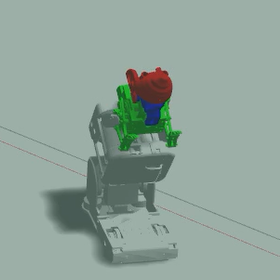
\includegraphics[width=3.0cm]{images/ch03/check/torear/0984.png}
  }
  \caption{Gazebo中生物鼠从初始姿态运动至直立姿态}\label{figure_simtorear}
\end{figure}

对机器鼠完成姿态切换所需时间的统计如表\ref{table_timeconsume}所示,表中$P_{0}$表示姿态切换的起始姿态,$P_{1}$表示姿态切换的目标姿态。
% \diagbox[width=1.8cm, height=1\line]{}{}

上述数据表明,机器鼠任意两种姿态之间切换所需时间均在$1.2~s$以内,能够满足行为交互的实时响应需求。

在运动精度方面,通过程序设定机械臂运动误差允许值为$0.001~rad$,动作执行层的接口函数保证了即使运动规划或执行过程中出现异常,系统也能迅速捕获并重新规划和执行,在这一条件下,系统稳定运行的时长超过$1~h$。表明仿真平台能够满足运动精度要求。
% \subsection{交互动作测试}
\begin{table}[htb]
  \linespread{1.5}
  \zihao{5}
  \centering
  \caption{机器鼠完成姿态切换所需时间(单位:$s$)}\label{table_timeconsume}
  \begin{tabular}{p{1.5cm}<{\centering\arraybackslash}|*{7}{>{\centering\arraybackslash}p{1.5cm}}}
    \toprule
    \diagbox[width=1.8cm, height=1.2\line]{$P_{0}$}{$P_{1}$} & 初始姿态 & 直立 & 嗅探 & 梳理  & 被梳理 & 攀爬 & 匍匐 \\ \midrule
    初始姿态 &  0  & 0.984  & 0.235 & 0.785 & 0.322  & 0.452 & 0.151  \\
    直立         & 0.897 &  0   & 0.725 & 0.668 & 1.052 & 0.735 & 1.034 \\
    嗅探         & 0.222 & 0.708  &  0  & 0.729 & 0.351  & 0.236 & 0.221  \\
    梳理         & 0.758 & 0.672  & 0.704 &  0  & 0.341  & 0.120 & 0.202  \\
    被梳理     & 0.335 & 0.989  & 0.350 & 0.352 &  0   & 0.330 & 0.104  \\
    攀爬         & 0.422 & 0.730  & 0.238 & 0.142 & 0.325  &  0  & 0.368  \\
    匍匐         & 0.162 & 1.125 & 0.210 & 0.215 & 0.132  & 0.327 &  0   \\
    \bottomrule
    \end{tabular}
\end{table}